\renewcommand{\tmpwidth}{36mm}
\newcommand{\tmpheight}{72mm}
\setlength{\tabcolsep}{2pt}
\begin{figure*}[!ht]
    \centering
    \begin{tabular}{c c c c}

   
    BigGAN (FID=$6.95$) & VQVAE-2$^\dagger$ (FID=$31$) & \model-8 (FID=\bestfid) & \model-64 (FID=5.14) \\
    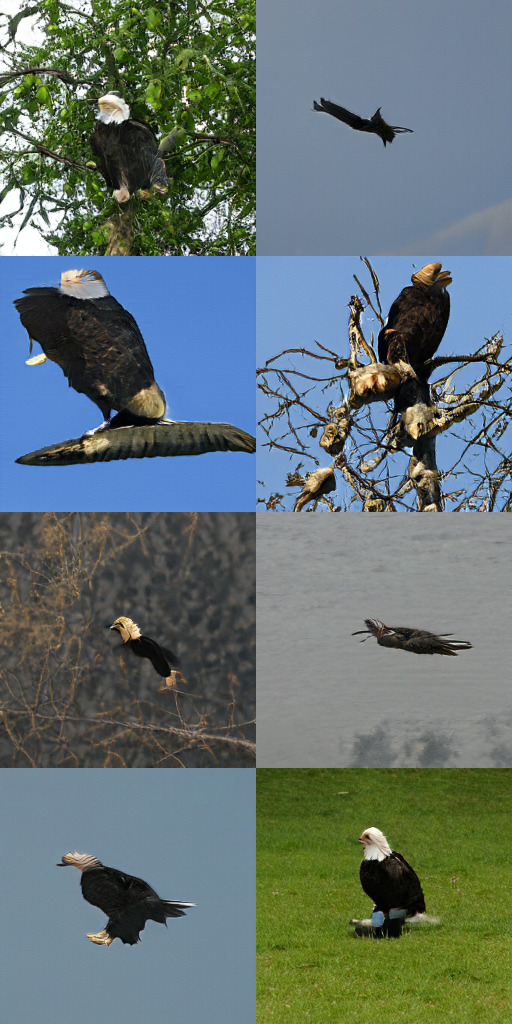
\includegraphics[width=\tmpwidth,  height=\tmpheight]{figures/supp_cc/22_bald-eagle_biggan.jpg} & 
    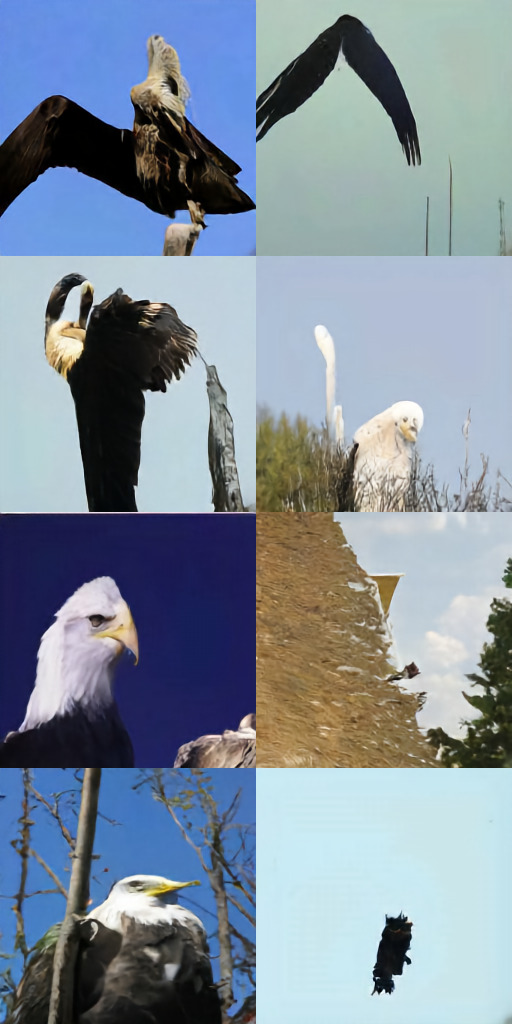
\includegraphics[ width=\tmpwidth, height=\tmpheight]{figures/supp_cc/22_bald-eagle_vqvae2.jpg} & 
    % 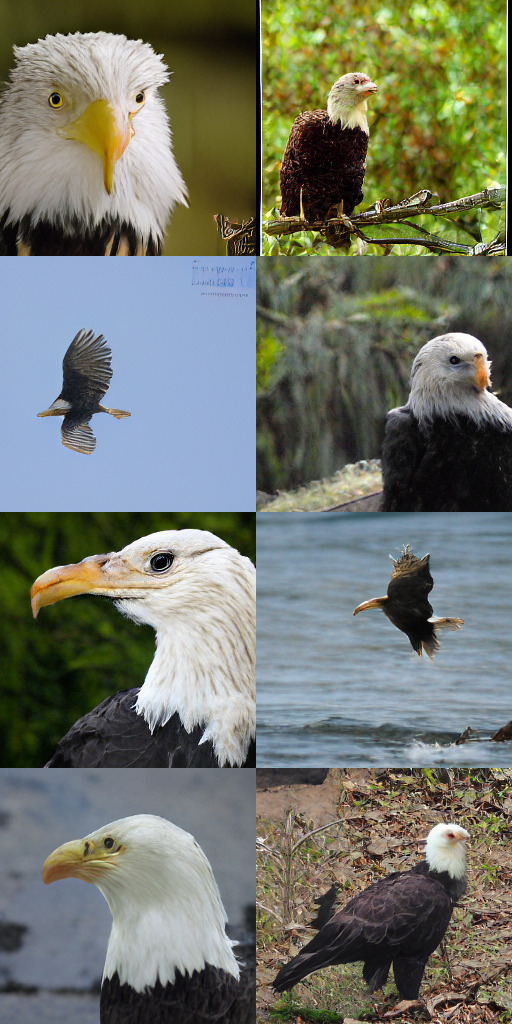
\includegraphics[ width=\tmpwidth, height=\tmpheight]{figures/supp_cc/22_bald-eagle_vqgan.jpg} & \ 
    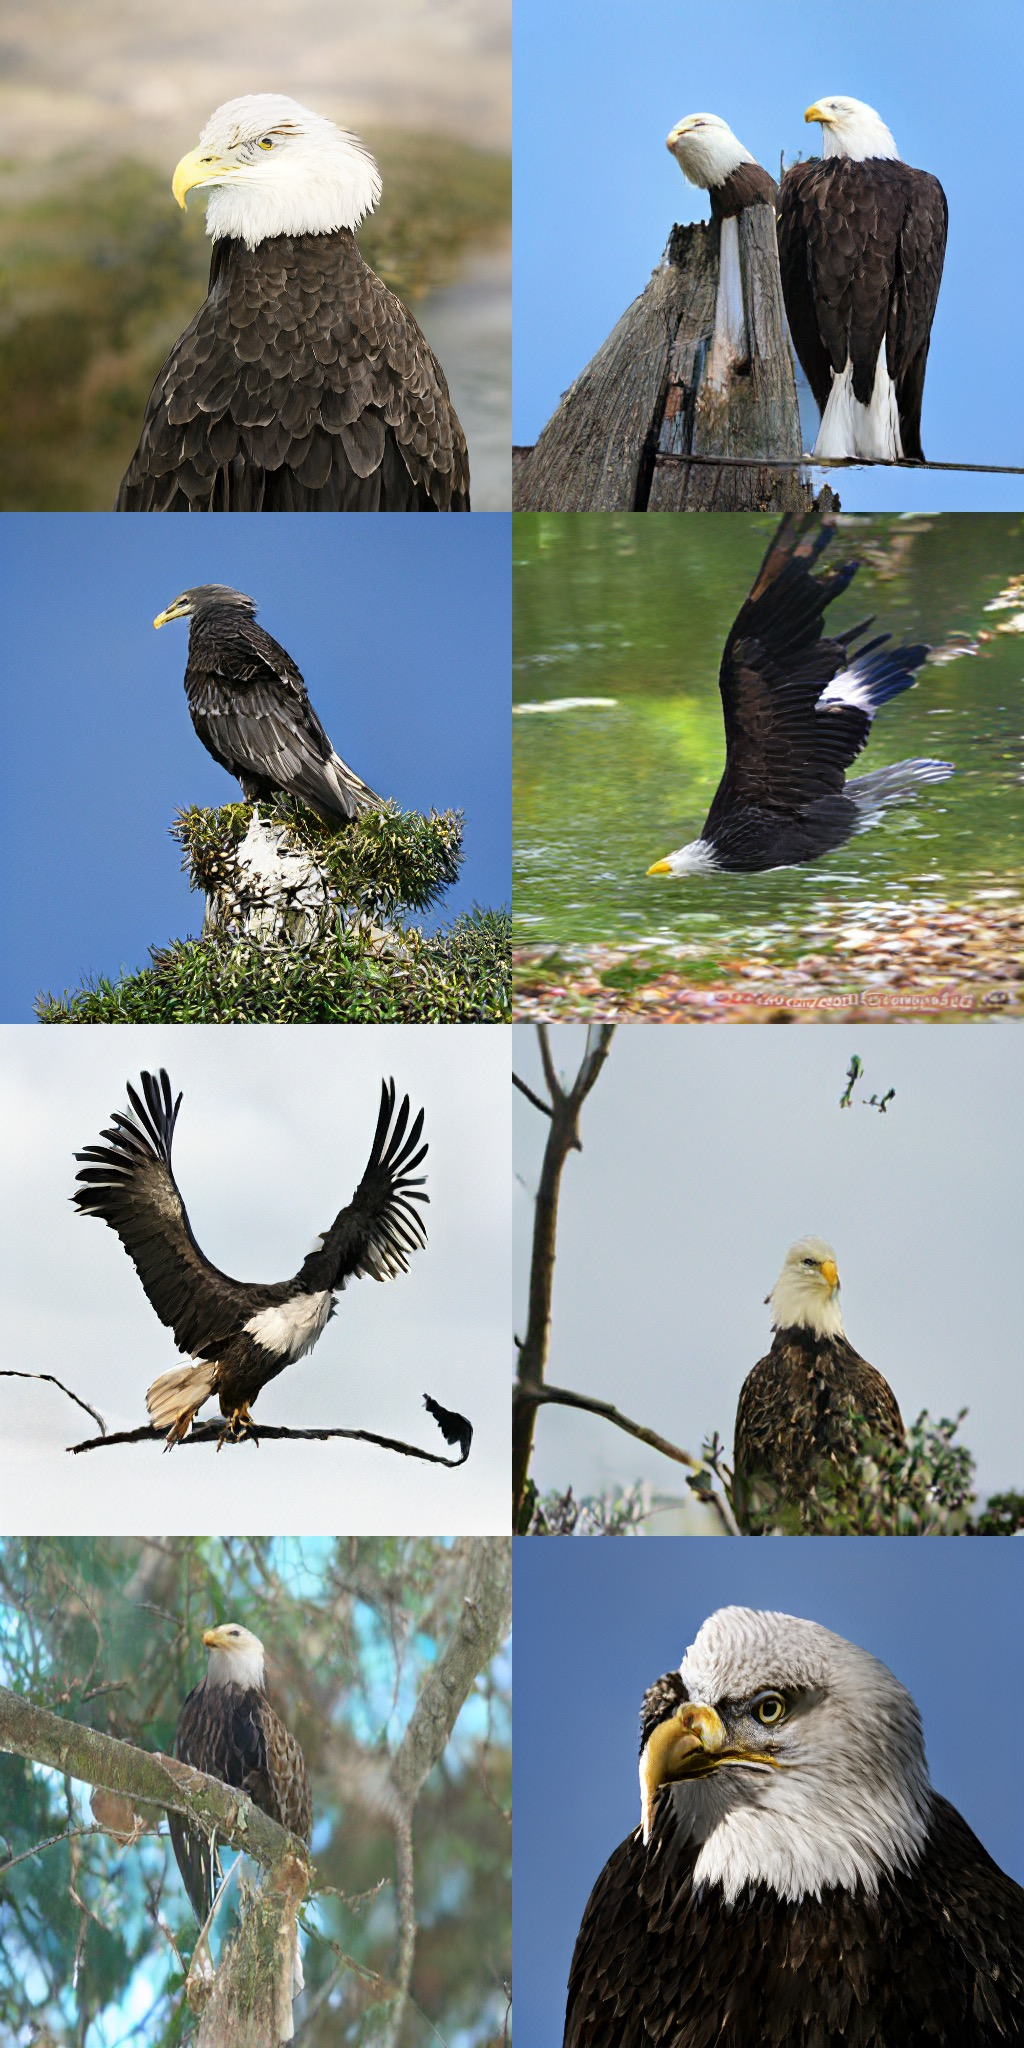
\includegraphics[ width=\tmpwidth, height=\tmpheight]{figures/supp_cc/22_bald-eagle_ours.png} &
    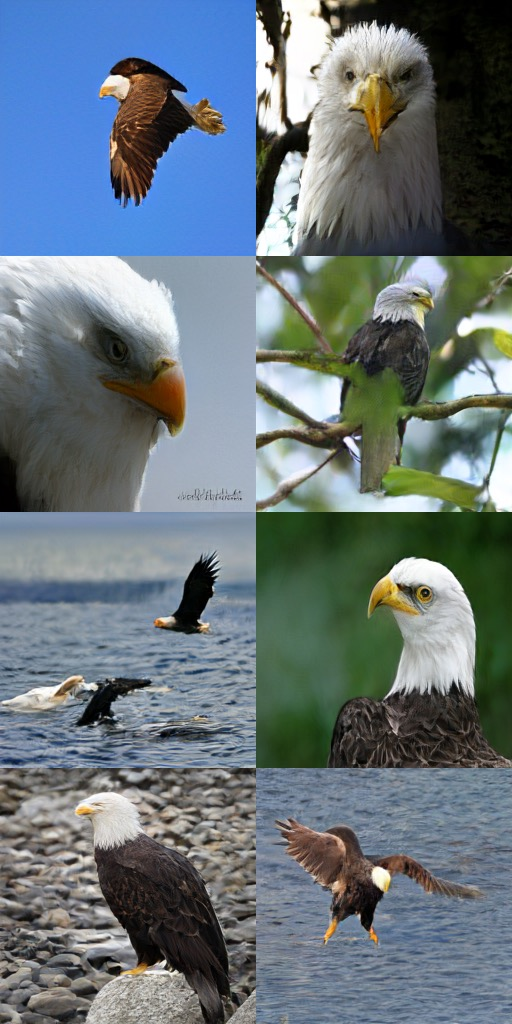
\includegraphics[ width=\tmpwidth, height=\tmpheight]{figures/supp_cc/22_bald-eagle_ours64.png}\\ 
       
    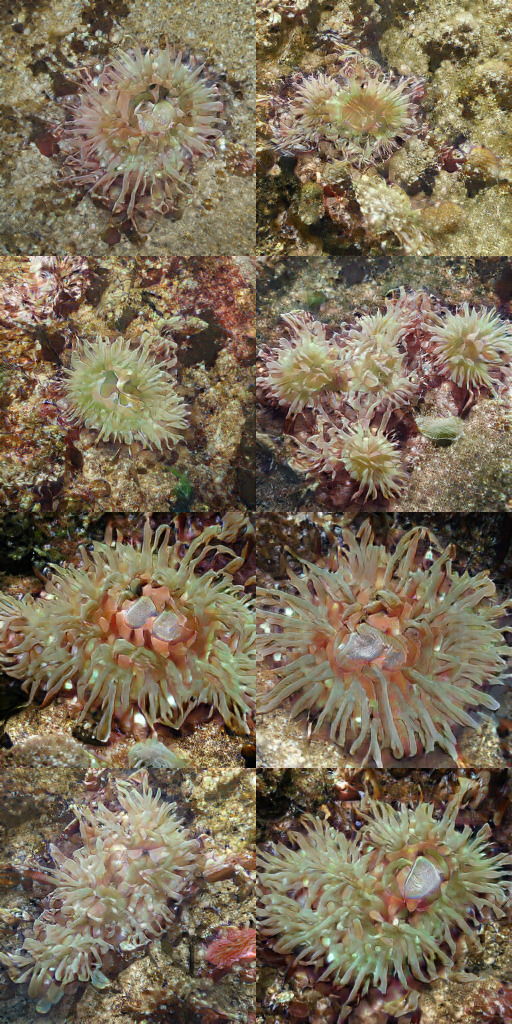
\includegraphics[ width=\tmpwidth, height=\tmpheight]{figures/supp_cc/108_anemone_biggan.jpg} & \
    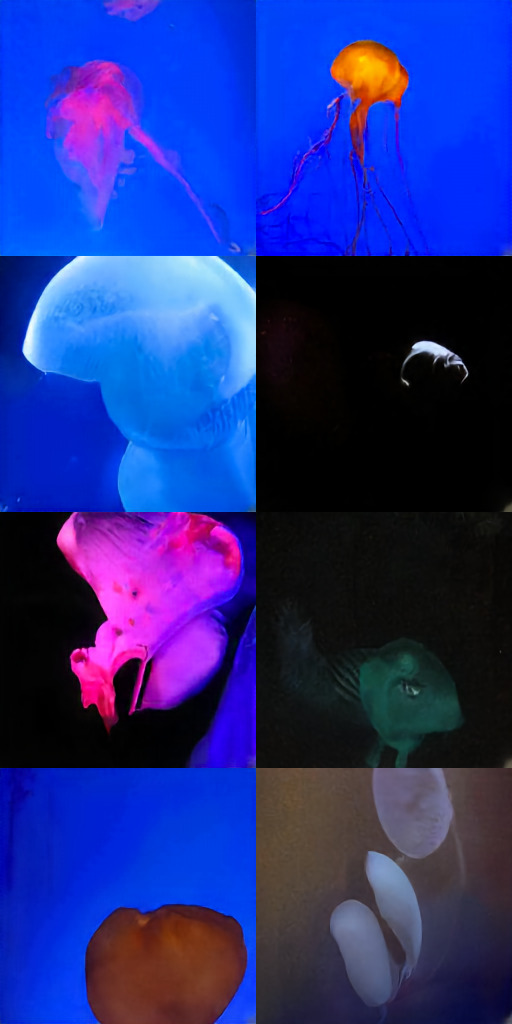
\includegraphics[ width=\tmpwidth, height=\tmpheight]{figures/supp_cc/108_anemone_vqvae2.jpg}& \
    % 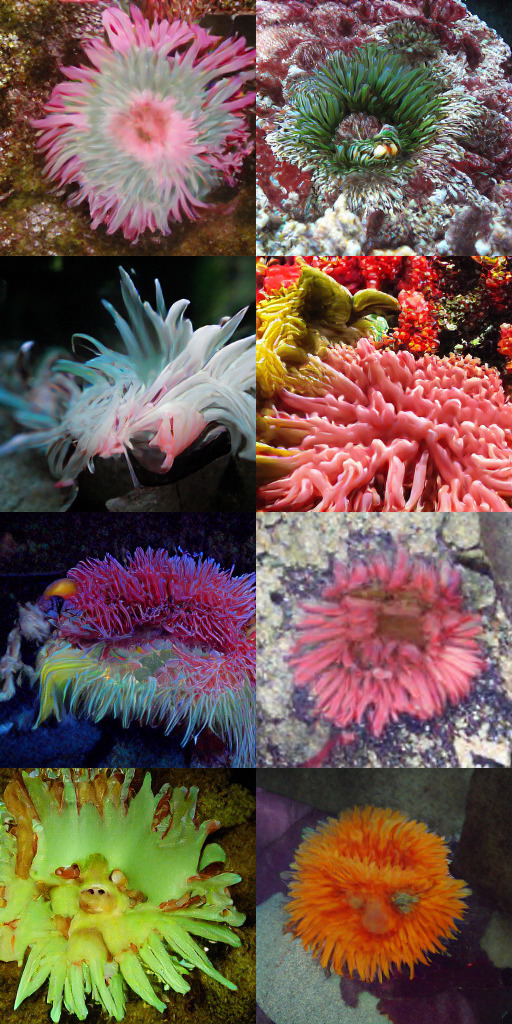
\includegraphics[ width=\tmpwidth, height=\tmpheight]{figures/supp_cc/108_anemone_vqgan.jpg} & \ 
    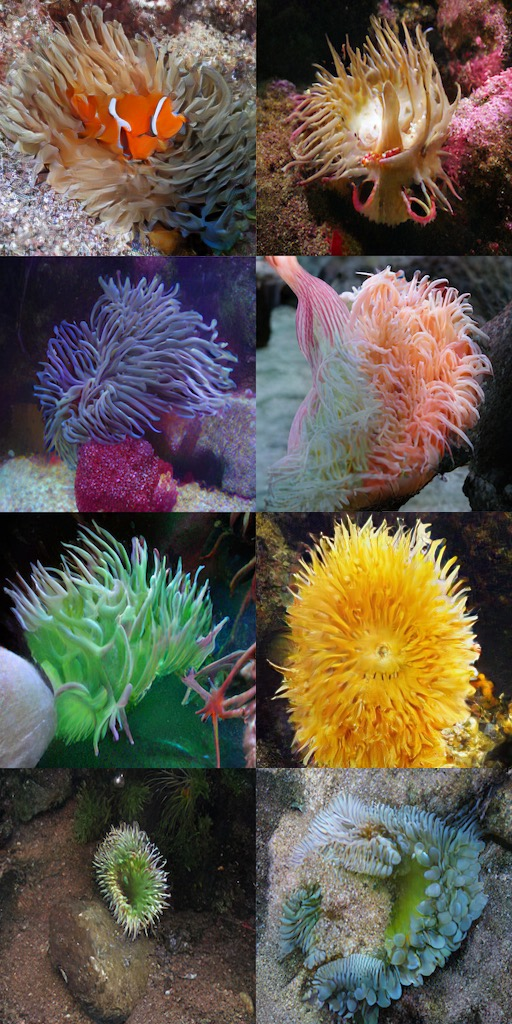
\includegraphics[ width=\tmpwidth, height=\tmpheight]{figures/supp_cc/108_anemone_ours.png} &
    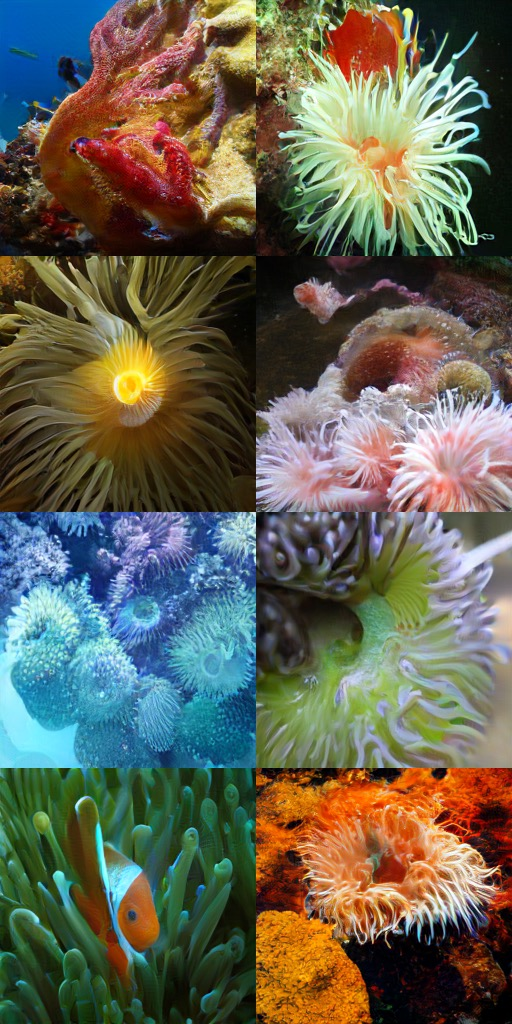
\includegraphics[ width=\tmpwidth, height=\tmpheight]{figures/supp_cc/108_anemone_ours64.png}\\ 
    
    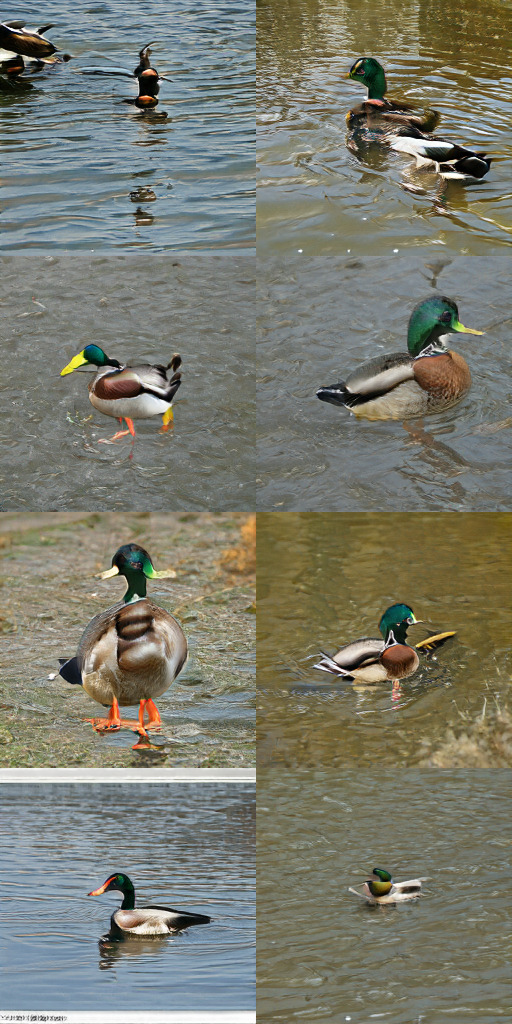
\includegraphics[ width=\tmpwidth, height=\tmpheight]{figures/supp_cc/97_drake_biggan.jpg} & \
    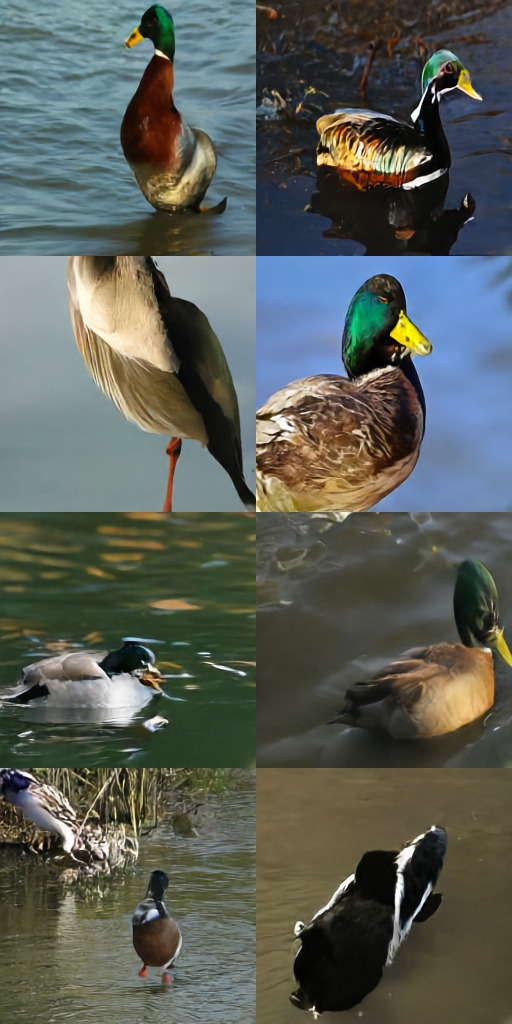
\includegraphics[ width=\tmpwidth, height=\tmpheight]{figures/supp_cc/97_drake_vqvae2.jpg}& \
    % 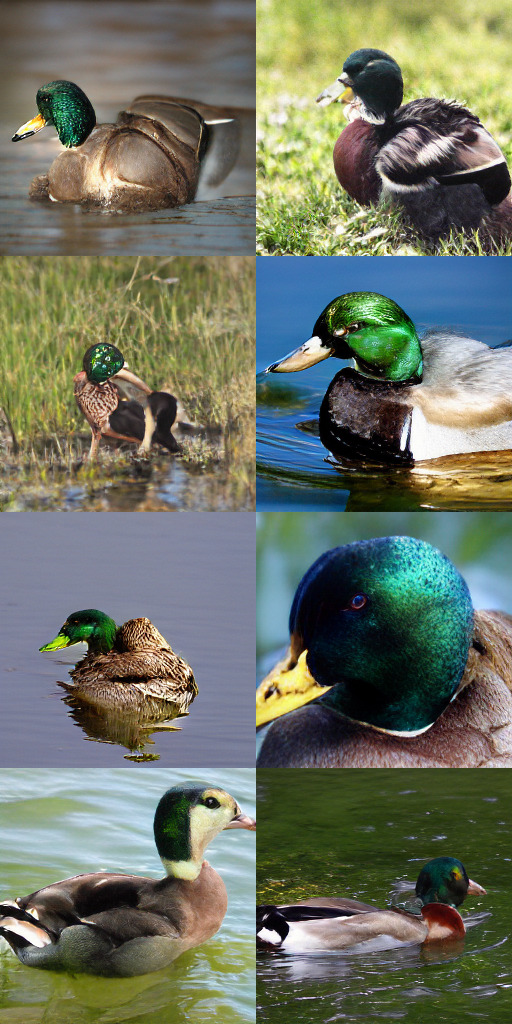
\includegraphics[ width=\tmpwidth, height=\tmpheight]{figures/supp_cc/97_drake_vqgan.jpg} & \ 
    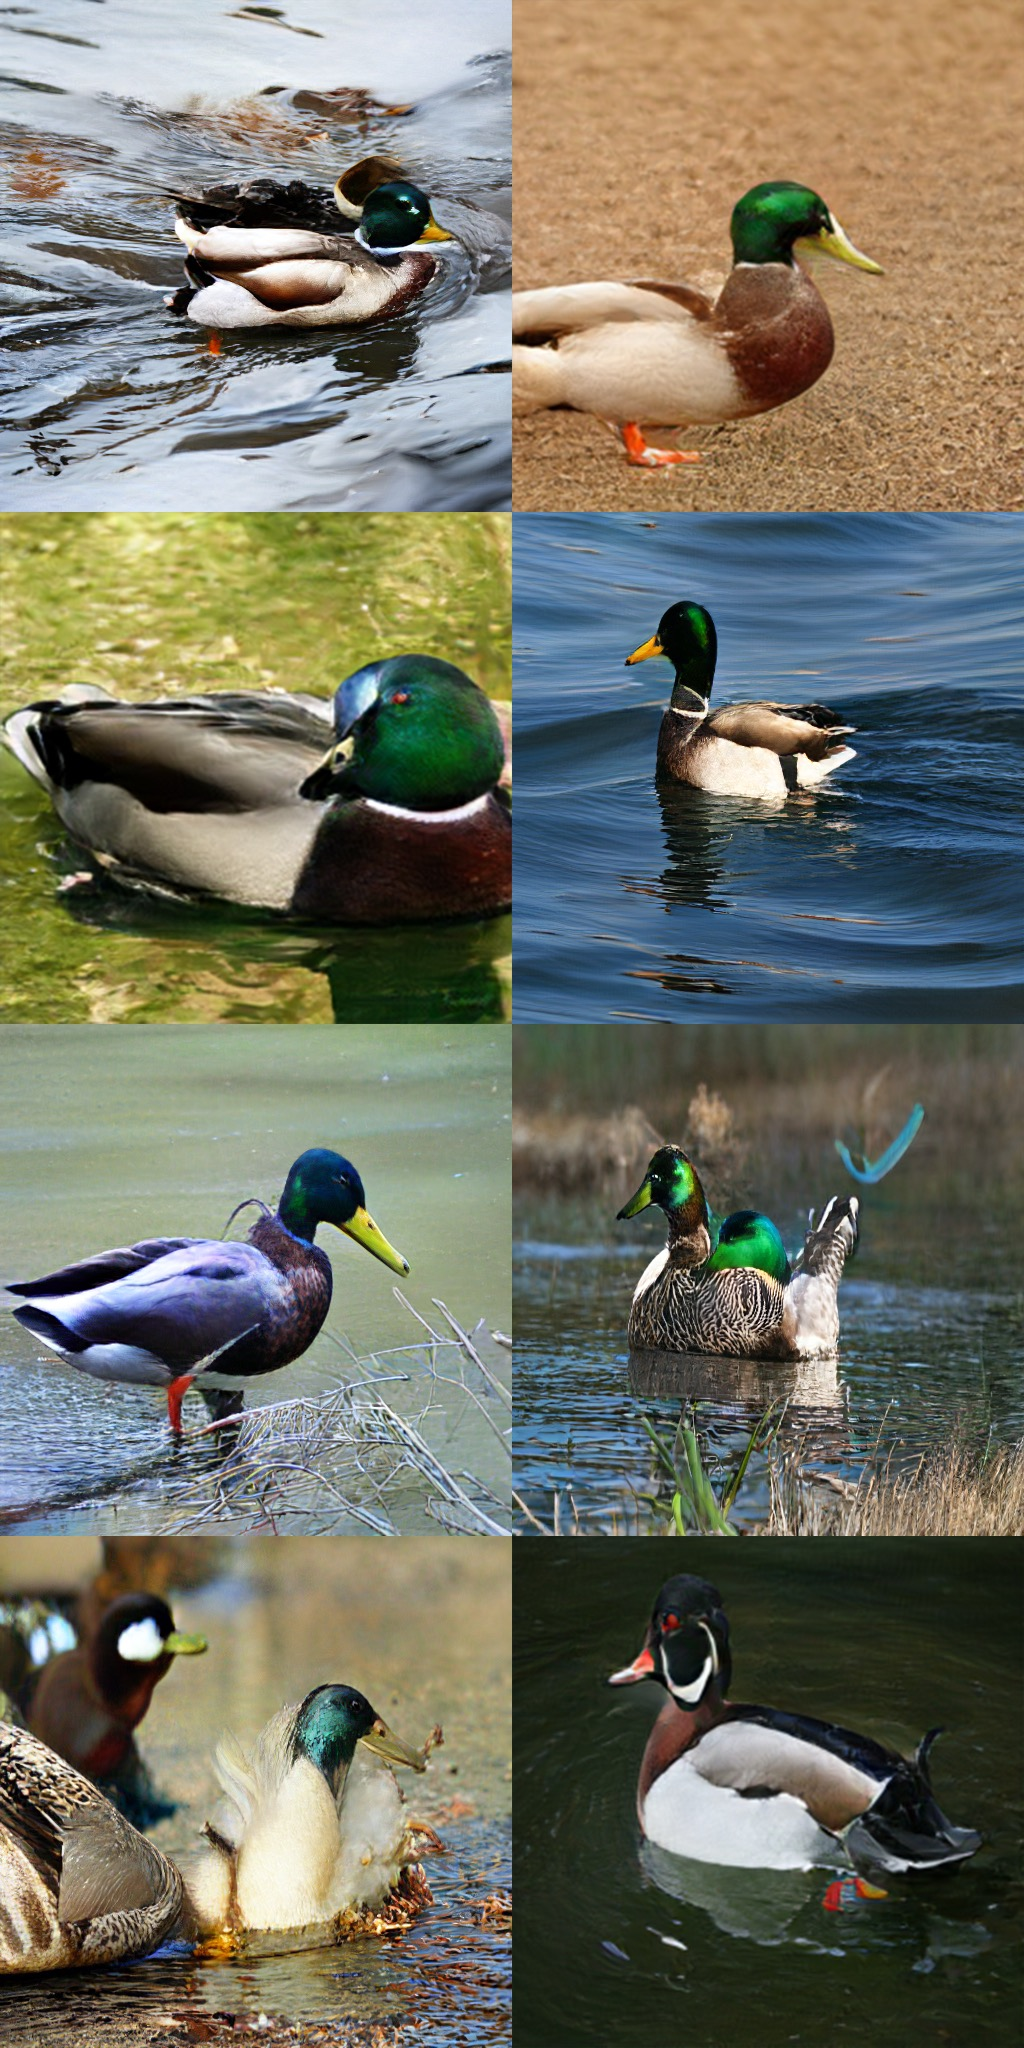
\includegraphics[ width=\tmpwidth, height=\tmpheight]{figures/supp_cc/97_drake_ours.png} & 
    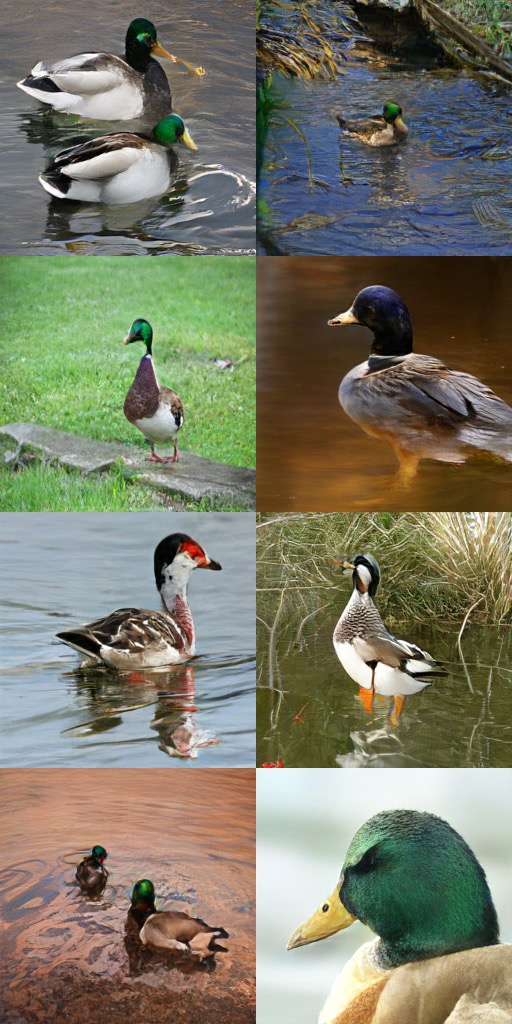
\includegraphics[ width=\tmpwidth, height=\tmpheight]{figures/supp_cc/97_drake_ours64.png}\\ 
        
    \end{tabular}
    \caption{\textbf{更多多样性比较}BigGAN-deep（截断$1.0$）、VQVAE-2和我们提出的方法\model在ImageNet上的比较。$^\dagger$表示从论文中提取的样本。}
    \vspace{-6mm}
    \label{fig:supp_cc_diversity0}
\end{figure*}
    
\begin{figure*}[!ht]
    \centering
    \begin{tabular}{c c c c}
    BigGAN (FID=$6.95$) & VQVAE-2$^\dagger$ (FID=$31$) & \model-8 (FID=\bestfid) & \model-64 (FID=5.14) \\
    
    % 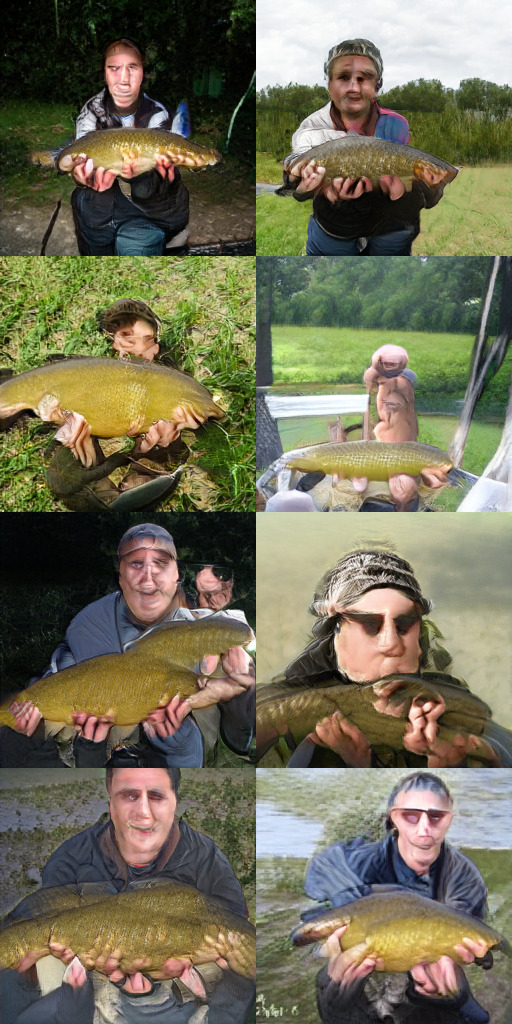
\includegraphics[ width=\tmpwidth, height=\tmpheight]{figures/supp_cc/0_tench_biggan.jpg} & \
    % 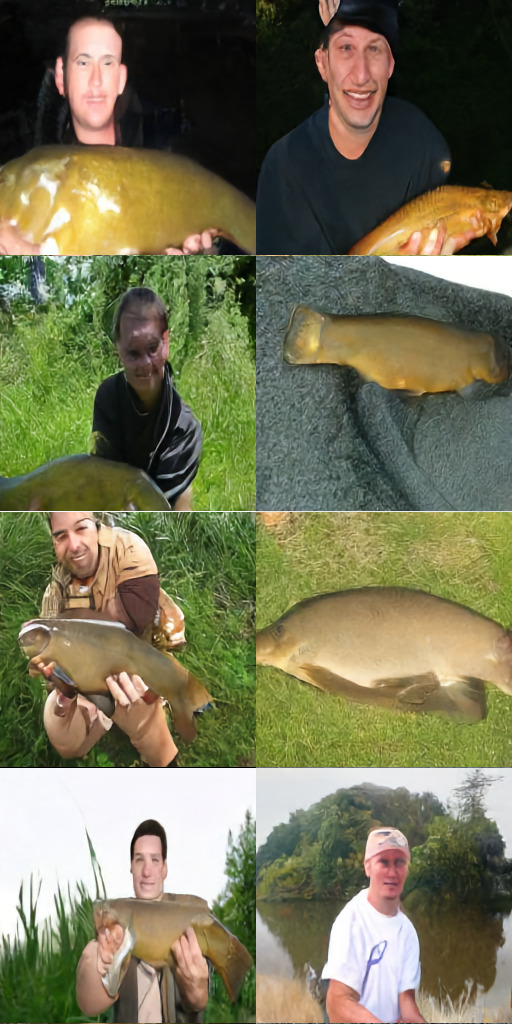
\includegraphics[ width=\tmpwidth, height=\tmpheight]{figures/supp_cc/0_tench_vqvae2.jpg}& \
    % % 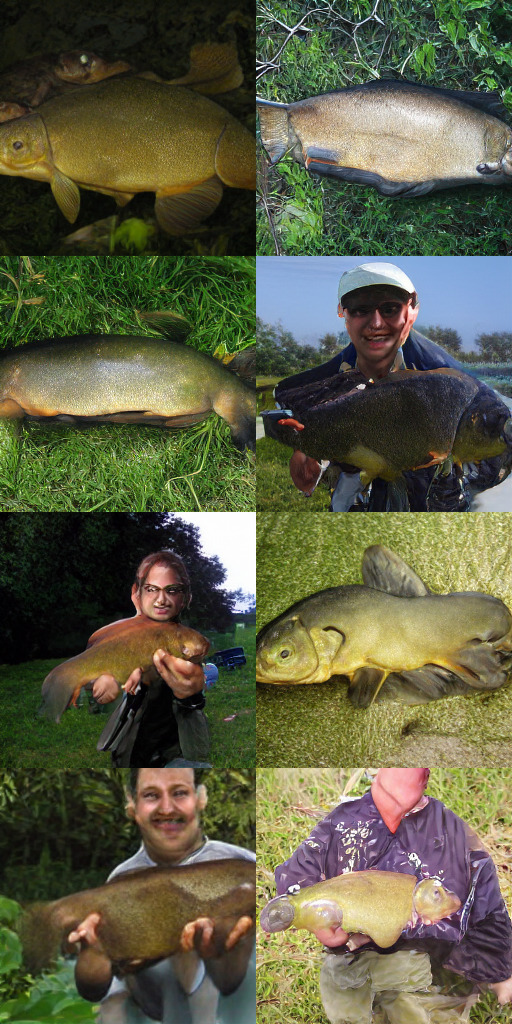
\includegraphics[ width=\tmpwidth, height=\tmpheight]{figures/supp_cc/0_tench_vqgan.jpg} & \ 
    % 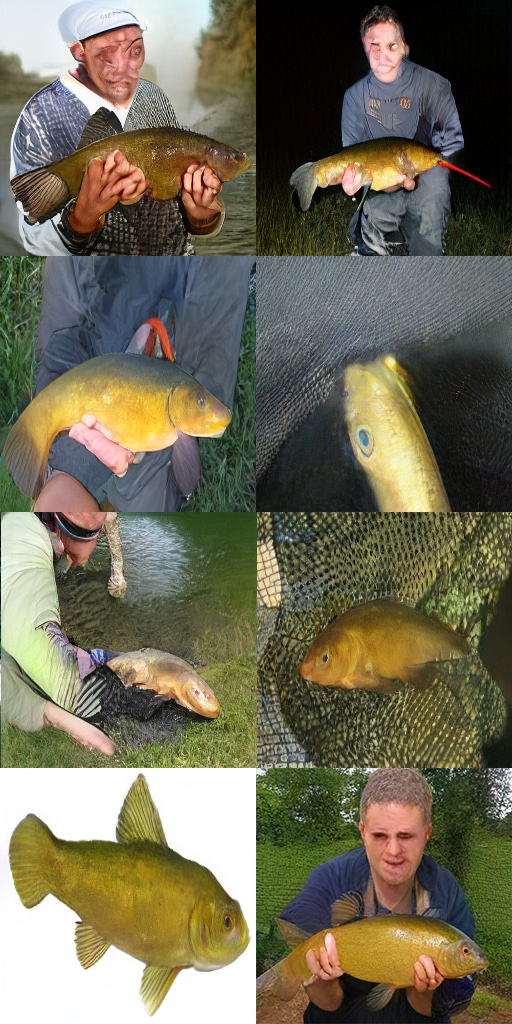
\includegraphics[ width=\tmpwidth, height=\tmpheight]{figures/supp_cc/0_tench_ours.png} \\ 

    % 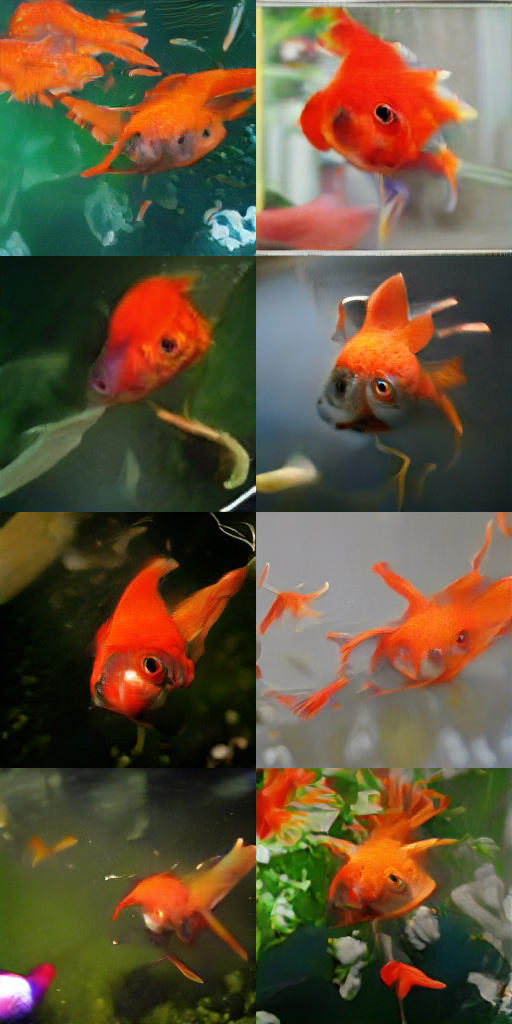
\includegraphics[ width=\tmpwidth, height=\tmpheight]{figures/supp_cc/1_goldfish_biggan.jpg} & \
    % 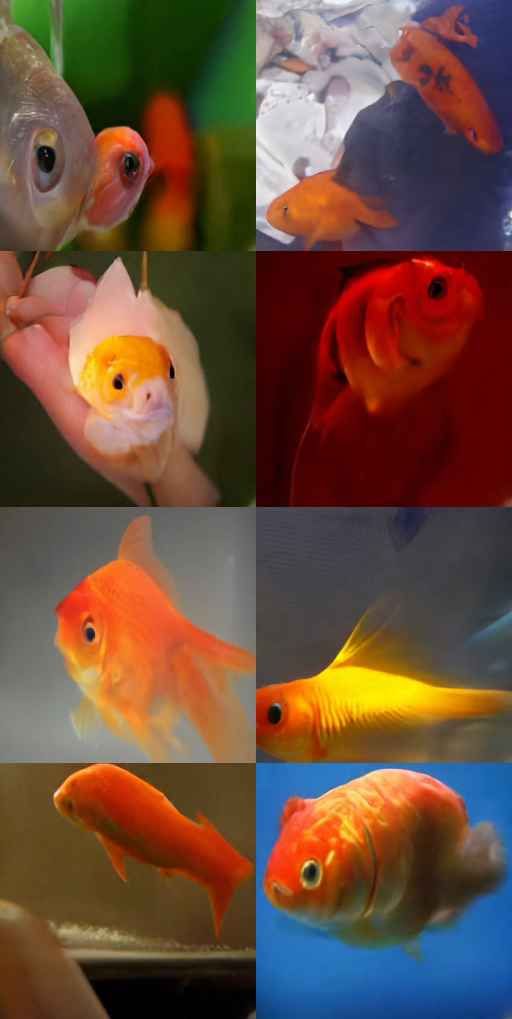
\includegraphics[ width=\tmpwidth, height=\tmpheight]{figures/supp_cc/1_goldfish_vqvae2.jpg}& \
    % 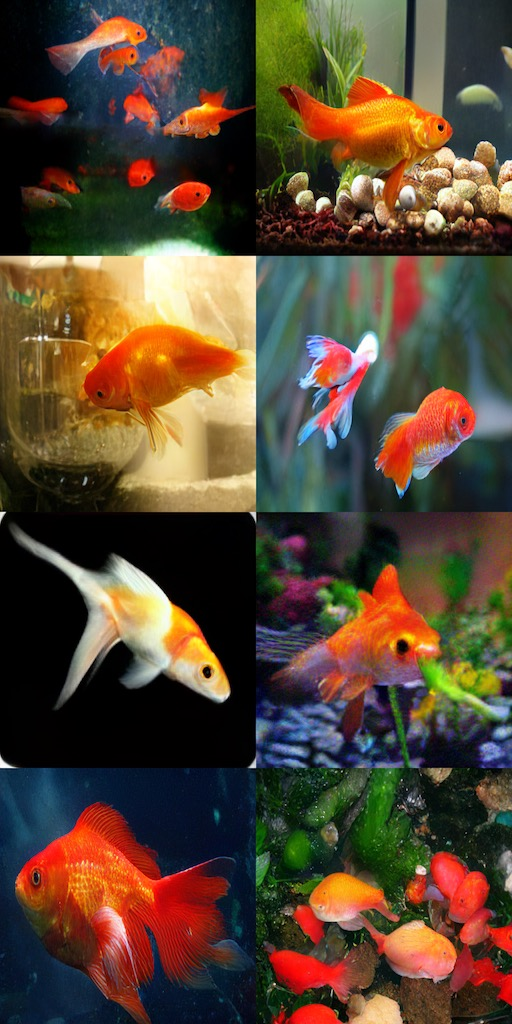
\includegraphics[ width=\tmpwidth, height=\tmpheight]{figures/supp_cc/1_goldfish_ours.png} \\ 
    
    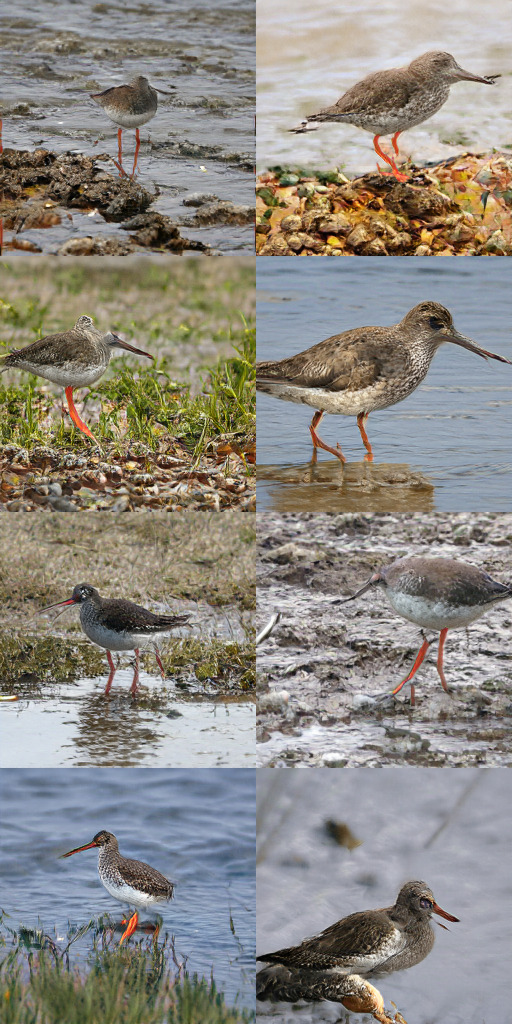
\includegraphics[ width=\tmpwidth, height=\tmpheight]{figures/supp_cc/141_redshank_biggan.jpg} & \
    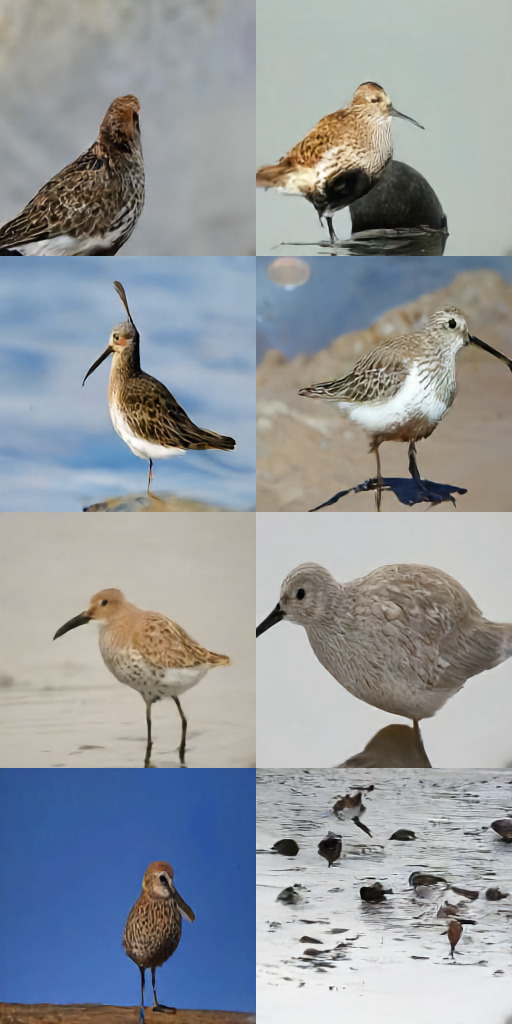
\includegraphics[ width=\tmpwidth, height=\tmpheight]{figures/supp_cc/141_redshank_vqvae2.jpg}& \
    % 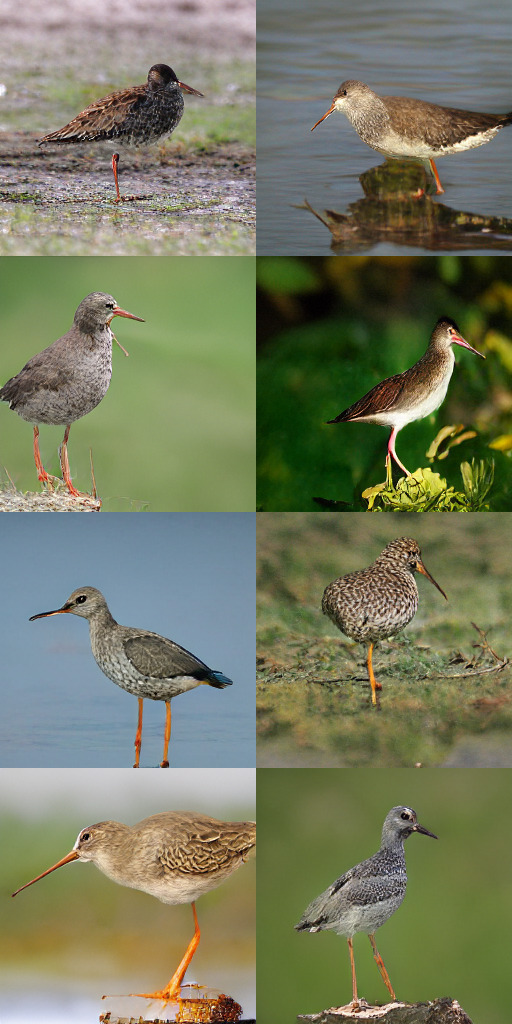
\includegraphics[ width=\tmpwidth, height=\tmpheight]{figures/supp_cc/141_redshank_vqgan.jpg} & \ 
    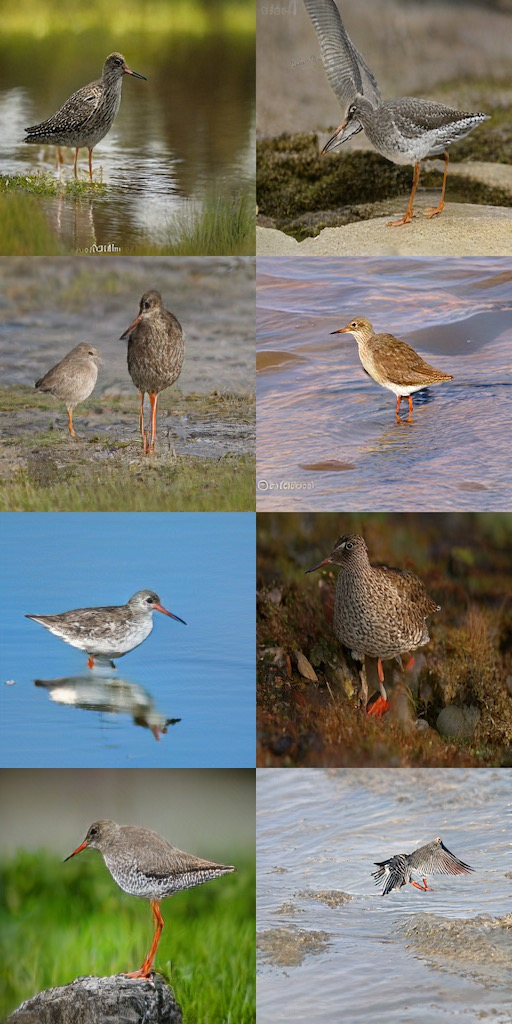
\includegraphics[ width=\tmpwidth, height=\tmpheight]{figures/supp_cc/141_redshank_ours.png} &
    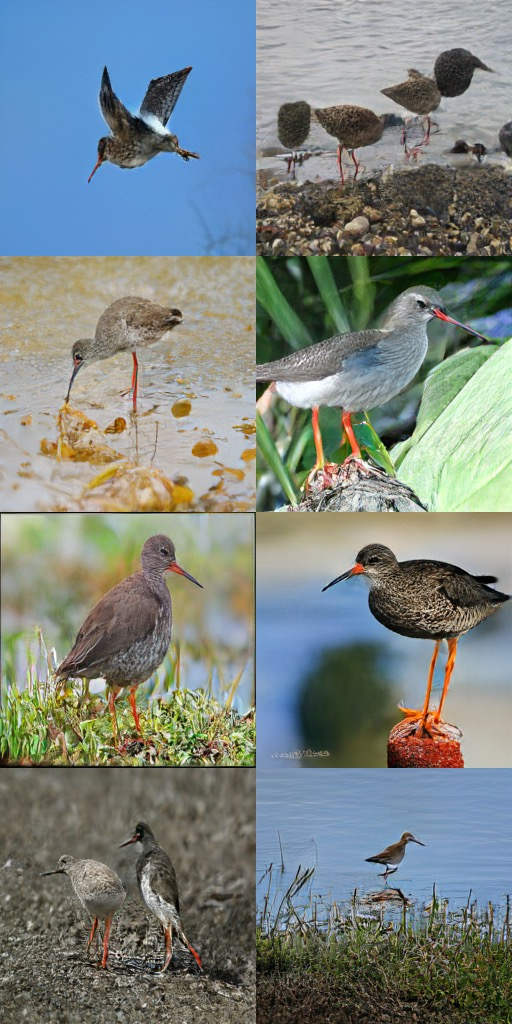
\includegraphics[ width=\tmpwidth, height=\tmpheight]{figures/supp_cc/141_redshank_ours64.png}\\ 
    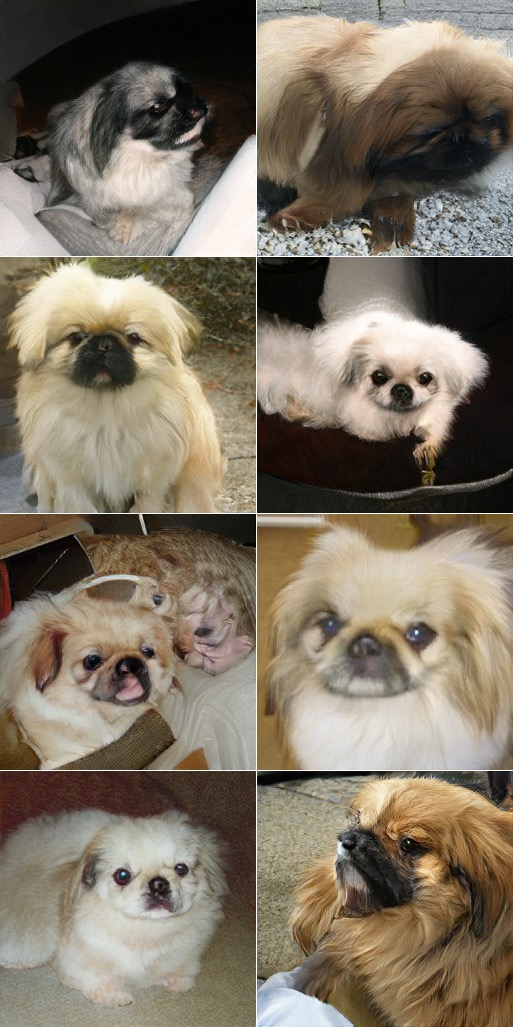
\includegraphics[ width=\tmpwidth, height=\tmpheight]{figures/supp_cc/154_biggan.png} & \
    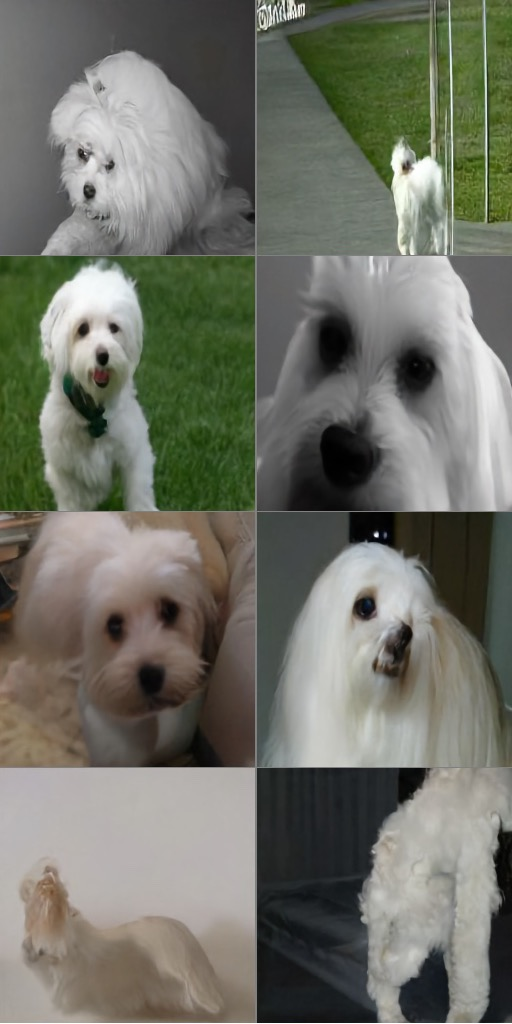
\includegraphics[ width=\tmpwidth, height=\tmpheight]{figures/supp_cc/154_vqvae2.png}& \
    % 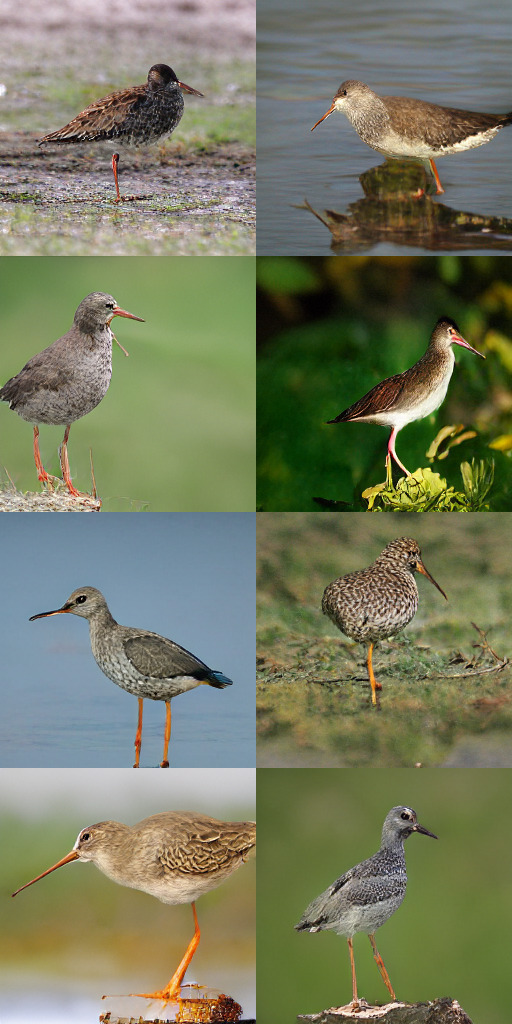
\includegraphics[ width=\tmpwidth, height=\tmpheight]{figures/supp_cc/141_redshank_vqgan.jpg} & \ 
    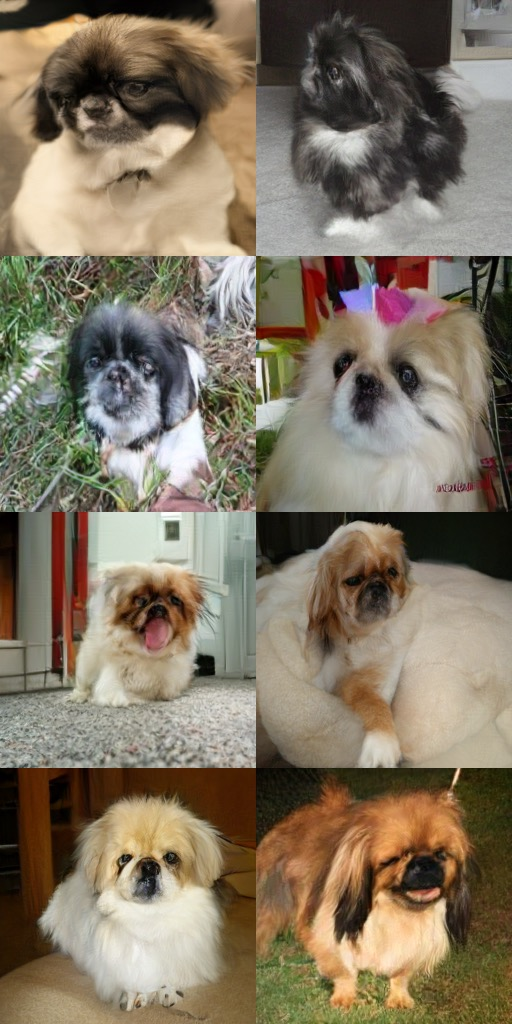
\includegraphics[ width=\tmpwidth, height=\tmpheight]{figures/supp_cc/154_ours8.png} &
    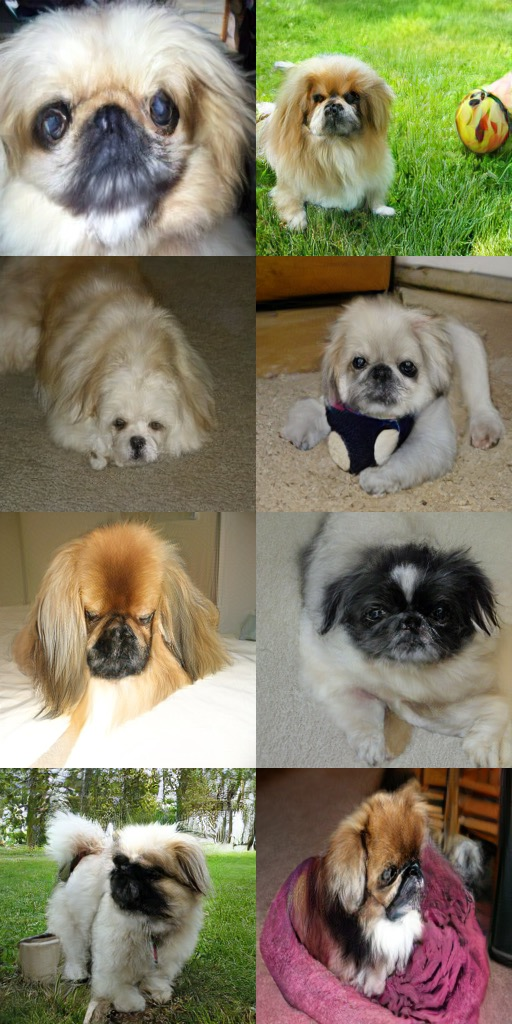
\includegraphics[ width=\tmpwidth, height=\tmpheight]{figures/supp_cc/154_ours64.png}\\ 

    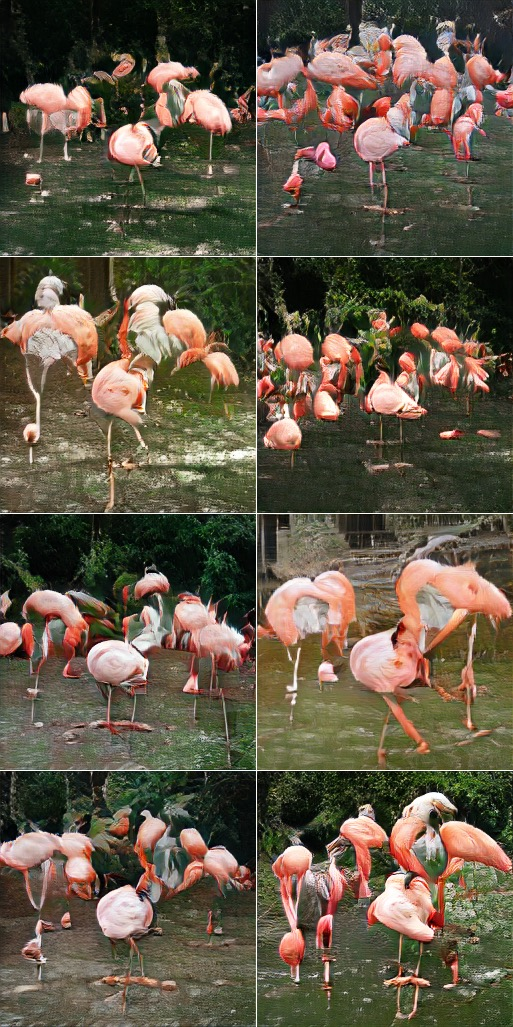
\includegraphics[ width=\tmpwidth, height=\tmpheight]{figures/supp_cc/130_flamingo_biggan.png} & \
    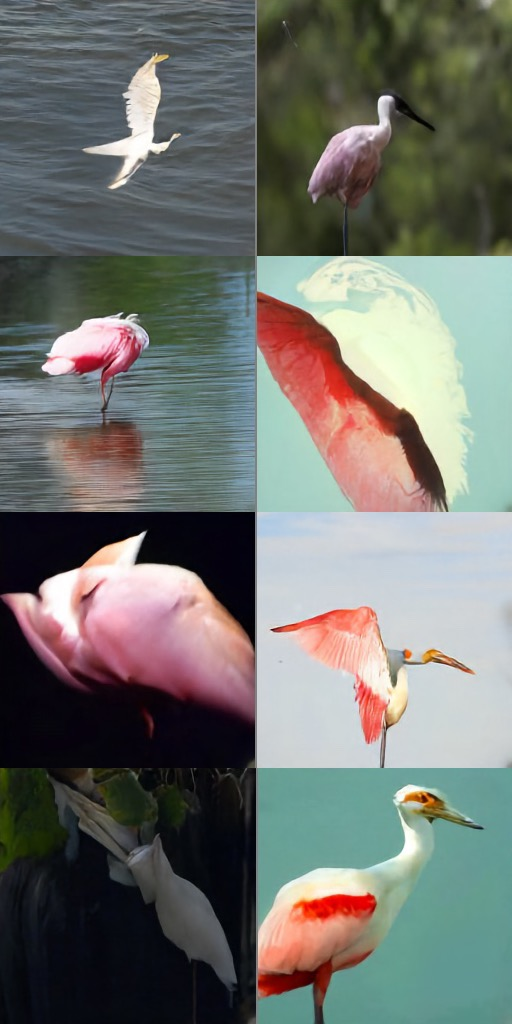
\includegraphics[ width=\tmpwidth, height=\tmpheight]{figures/supp_cc/130_flamingo_vqvae2.png}& \
    % 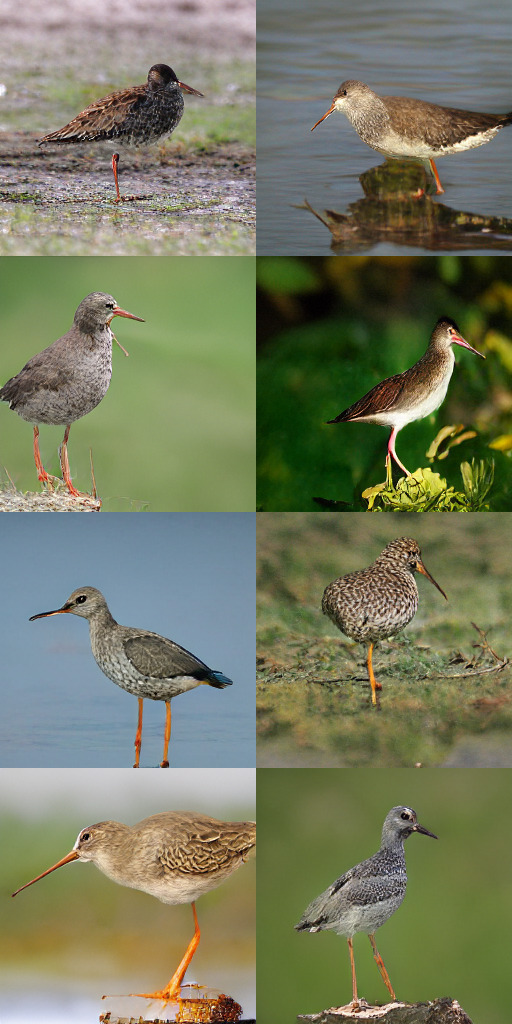
\includegraphics[ width=\tmpwidth, height=\tmpheight]{figures/supp_cc/141_redshank_vqgan.jpg} & \ 
    
    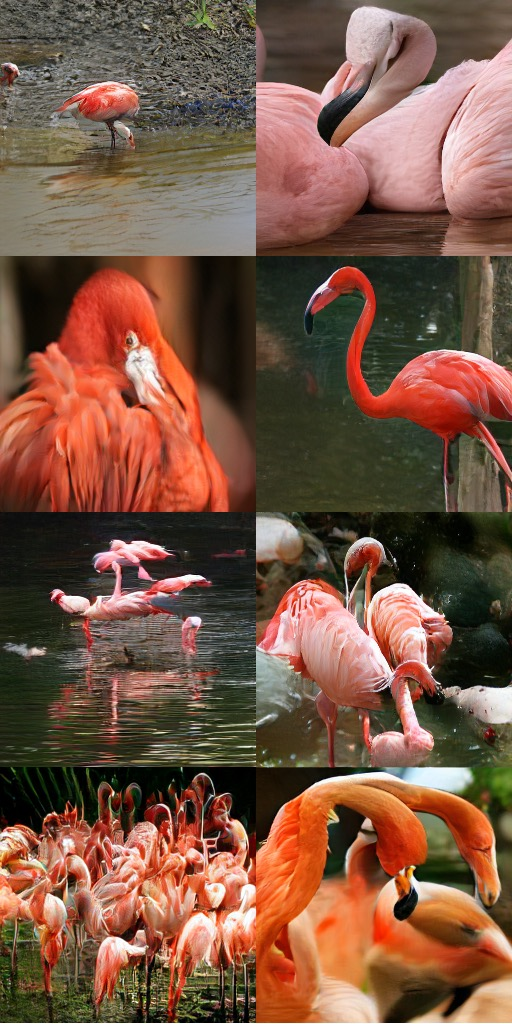
\includegraphics[ width=\tmpwidth, height=\tmpheight]{figures/supp_cc/130_flamingo_ours8.png} &
    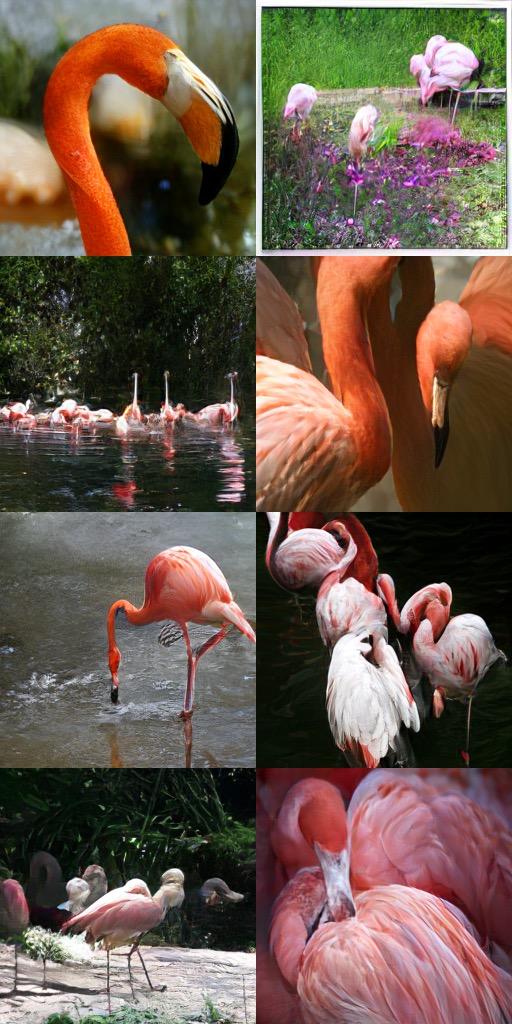
\includegraphics[ width=\tmpwidth, height=\tmpheight]{figures/supp_cc/130_flamingo_ours64.png} \\ 
\end{tabular}
    \caption{BigGAN-deep（截断$1.0$）、VQVAE-2和我们提出的方法\model在ImageNet上的更多多样性比较。$^\dagger$表示从论文中提取的样本。}
    \vspace{-6mm}
    \label{fig:supp_cc_diversity2}
\end{figure*}